%%----------------------------------------------------------------------------
%% Onderzoekstechnieken: Analyse van 2 kwalitatieve variabelen
%%----------------------------------------------------------------------------

\documentclass[aspectratio=169]{beamer}

%==============================================================================
% Aanloop
%==============================================================================

%---------- Vormgeving --------------------------------------------------------

\usetheme{hogent}

\usecolortheme{hgwhite} % witte achtergrond, zwarte tekst

\usepackage{graphicx,multicol}
\usepackage{comment,enumerate,hyperref}
\usepackage{amsmath,amsfonts,amssymb}
\usepackage[dutch]{babel}
\usepackage{multirow}
\usepackage{eurosym}
\usepackage{listings}
\usepackage{textcomp}
\usepackage{framed}
\usepackage{wrapfig}
\usepackage{tabu} %needed for \tabulinesep
\usepackage{wrapfig}
\usepackage{pgf-pie}
\usepackage{pgfplots}
\usepackage{booktabs}
\usepackage{pgfplotstable}
\usepackage{changepage}
\usepackage{ulem} % for \sout{text} (strikethrough)
\usepackage{fancyvrb} % for \begin{Verbatim} (LaTeX controls within verbatim)
\usepackage[output-decimal-marker={,}]{siunitx} 

%---------- Configuratie ------------------------------------------------------

\pgfplotsset{compat=1.16}
\usetikzlibrary{arrows,shapes,backgrounds,positioning,shadows}
\usetikzlibrary{pgfplots.statistics}

%---------- Commando-definities -----------------------------------------------

\newcommand{\tabitem}{~~\llap{\textbullet}~~}
\newcommand{\alertbox}[2][hgblue]{%
  \setbeamercolor{alertbox}{bg=#1,fg=white}
  \begin{beamercolorbox}[sep=2pt,center]{alertbox}
    \textbf{#2}
  \end{beamercolorbox}
}
\pgfmathdeclarefunction{gauss}{2}{%
  \pgfmathparse{1/(#2*sqrt(2*pi))*exp(-((x-#1)^2)/(2*#2^2))}%
}

%---------- Info over de presentatie ------------------------------------------

\title{Chapter 6. Bivariate Analysis: qualitative - qualitative}
\subtitle{Research Techniques}
\author{Jens Buysse \and Pieter-Jan Maenhaut \and Bert {Van Vreckem}}
\date{AY 2020-2021}

%==============================================================================
% Inhoud presentatie
%==============================================================================

\begin{document}

\begin{frame}
  \maketitle
\end{frame}

\begin{frame}
  \frametitle{What's on the menu?}
  
  \tableofcontents
\end{frame}

\begin{frame}
  \frametitle{Learning Goals}
  
  \begin{itemize}
    \item Dependent/independent variable
    \item Apply suitable analysis techniques for each combination of measurement levels
    \item Crosstables and Cramér's $V$
    \item Visualization
  \end{itemize}
\end{frame}

\begin{frame}
  \frametitle{Overview}
    \centering
    \begin{tabular}{lll}
      \toprule
      \textbf{Independent}    & \textbf{Dependent}    & \textbf{Test/Metric}          \\
      \midrule
      Qualitative             & Qualitative           & $\chi^2$-test                 \\
                              &                       & Cramér's $V$                  \\
      Qualitative             & Quantitative          & two-sample $t$-test           \\
    	                        &                       & Cohen's $d$                   \\
      Quantitative            & Quantitative          & ---                           \\
    	                        &                       & Regression, correlation       \\
    	\bottomrule
    \end{tabular}
\end{frame}

\section{Bivariate analysis}

\begin{frame}
  \frametitle{Bivariate Analyse}
  \note{This slide is used to giva an example of a less trivial relationship between variables: Ant Colony optimization. Possible relationships between variables:
    
    \begin{itemize}
      \item The number of obstacles between the ant nest and the food source
      \item Algorithm used for removing / adding pheromones
      \item The shape of the obstacles between the nest and source
      \item \dots
  \end{itemize}}
  \begin{figure}
    \centering
    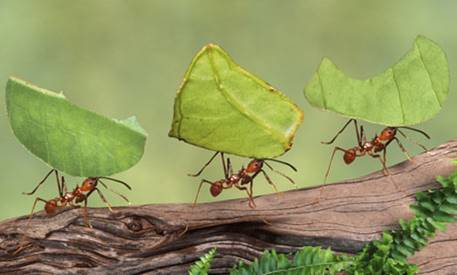
\includegraphics[width=0.8\textwidth]{ants.jpg}
    \label{fig:ants}
  \end{figure}
  
\end{frame}

\begin{frame}
  \frametitle{Example}
  \framesubtitle{Survey college restaurant visitors}
  
  \begin{itemize}
    \item How often do people visit the restaurant?
    \item Is there a difference in spending between students and staff?
    \item Is there a relationship between the number of visits and the total amount spent per week?
  \end{itemize}
  
  R Code: cfr. \texttt{syllabus/data/catering\_hogeschool.R}
  
  \centering
  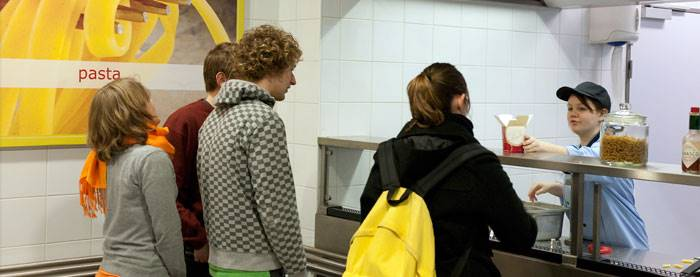
\includegraphics[height=.4\textheight]{students.jpg}
\end{frame}

\begin{frame}{How often do people visit the restaurant?}
  \begin{columns}
    \begin{column}{0.5\textwidth}
      \begin{table}[h]
        \small
        \begin{tabular}{|l|l|}
          \hline
          { \textbf{Statistic}}  & \textbf{Value}  \\ \hline
          Mean                   & 2.96            \\ \hline
          Median                 & 3               \\ \hline
          Mode                   & 2               \\ \hline
          Stdev                  & 1.484           \\ \hline
          Variance               & 2.202           \\ \hline
          Range                  & 4               \\ \hline
          $Q_{1}$                & 2               \\ \hline
          $Q_{2}$                & 3               \\ \hline
          $Q_{3}$                & 5               \\ \hline
        \end{tabular}
      \end{table}
    \end{column}
    \begin{column}{0.5\textwidth}
      
      \begin{figure}
        \centering
        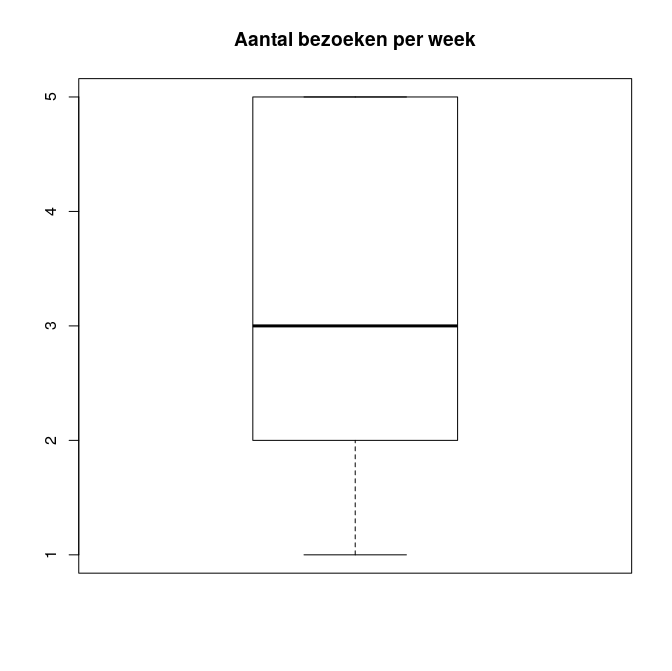
\includegraphics[height=.8\textheight]{2var-boxplot-aantalbezoeken}
        \label{fig:boxplotStudenten}
      \end{figure}
      
    \end{column}
  \end{columns}
\end{frame}

\begin{frame}{How often do people visit the restaurant?}
  
  \begin{columns}
    
    \begin{column}{0.5\textwidth}
      \begin{figure}
        \centering
        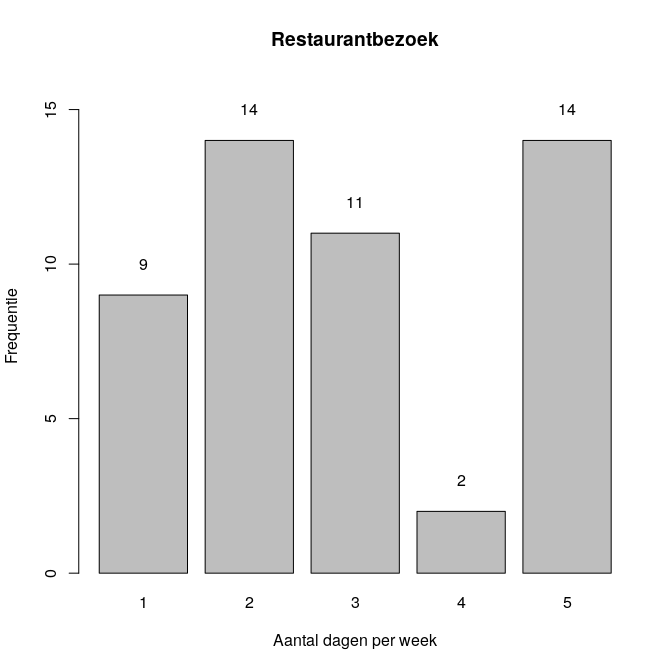
\includegraphics[height=.8\textheight]{2var-barplot-aantalbezoeken}
        \label{fig:studentenbar}
      \end{figure}
    \end{column}
    
    \begin{column}{0.5\textwidth}
      \begin{figure}
        \centering
        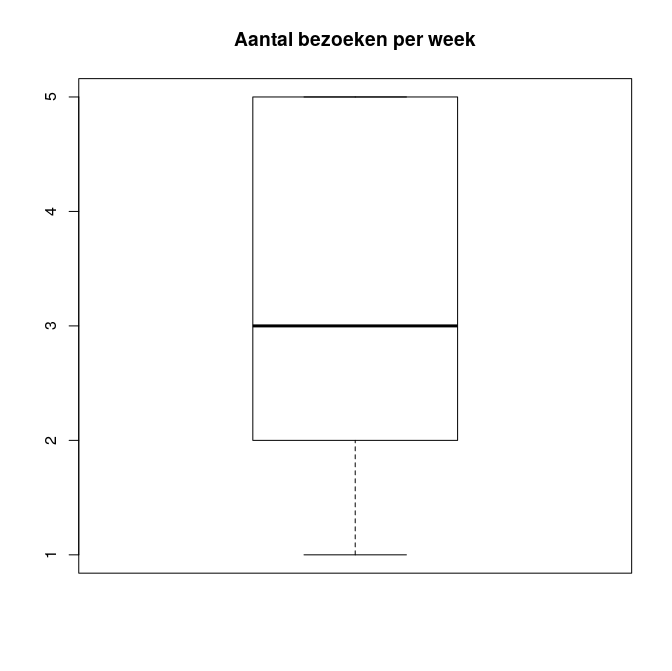
\includegraphics[height=.8\textheight]{2var-boxplot-aantalbezoeken}
        \label{fig:boxplotStudenten2}
      \end{figure}
    \end{column}
    
  \end{columns}
\end{frame}

\begin{frame}{Student vs Staff}
  
  \begin{itemize}
    \item \alert<1>{Single bar chart} (of mean per category)
    \item \alert<2>{Boxplot}
  \end{itemize}
  
  \begin{figure}
    \centering
    \only<1>{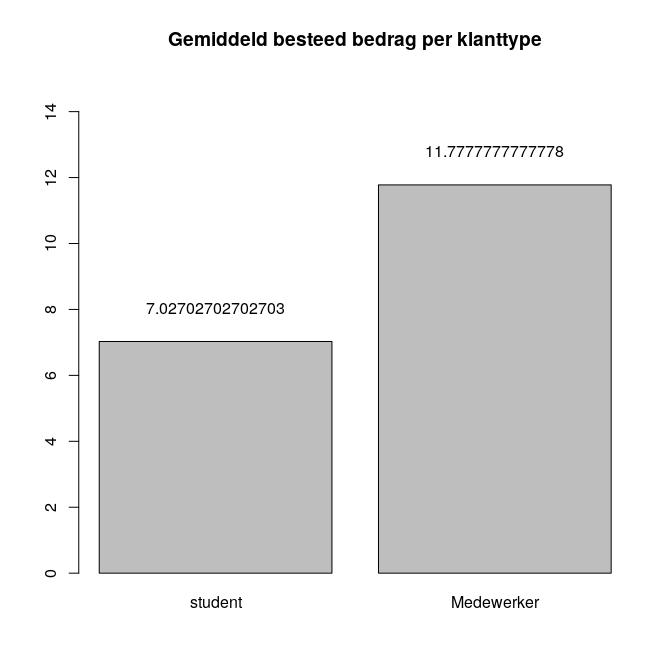
\includegraphics[height=0.6\textheight]{2var-barplot-gemiddeld-bedrag}}
    \only<2>{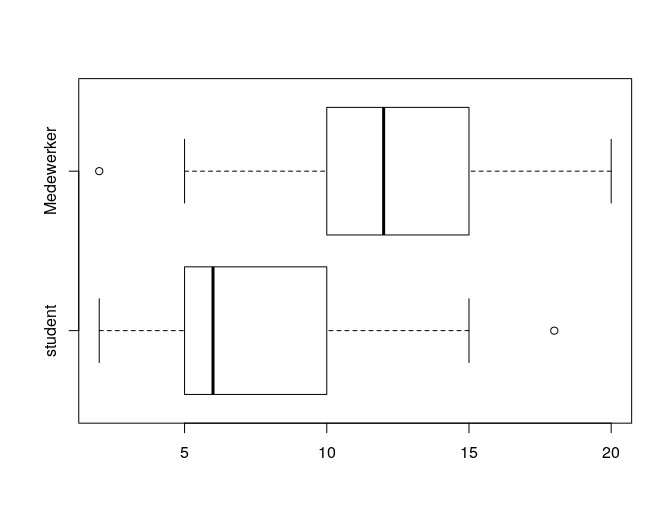
\includegraphics[height=0.6\textheight]{2var-boxplot-klanttype-bedrag}}
  \end{figure}
  
  \only<1>{\textbf{Note!} Insufficient to demonstrate a significant difference!}
\end{frame}

\begin{frame}
  \frametitle{Dependent and independent variable}
  
  \begin{columns}
    \begin{column}{0.3\textwidth}
      
      \begin{figure}
        \centering
        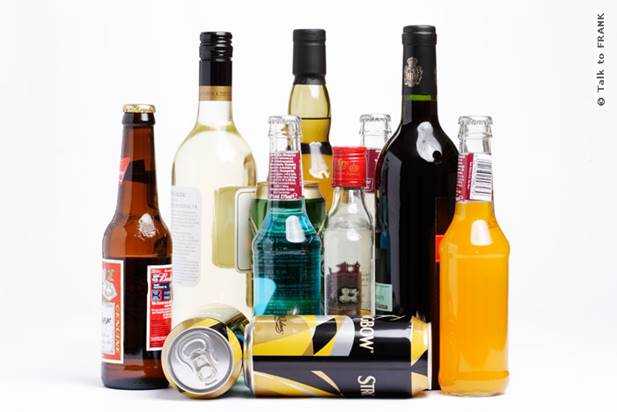
\includegraphics[width=1.00\textwidth]{liquor.jpg}
        \label{fig:liquor}
      \end{figure}
      
    \end{column}
    \begin{column}{0.3\textwidth}
      
      \begin{figure}
        \centering
        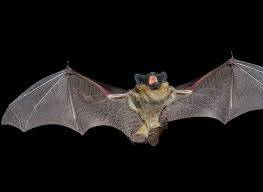
\includegraphics[width=1.00\textwidth]{bat.jpg}
        \label{fig:bat}
      \end{figure}
      
    \end{column}
    \begin{column}{0.3\textwidth}
      
      \begin{figure}
        \centering
        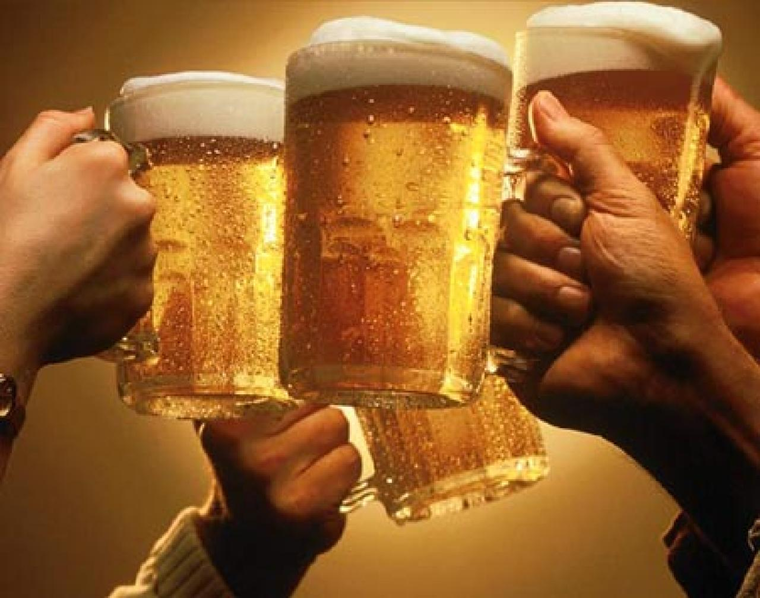
\includegraphics[width=1.00\textwidth]{beer.png}
        \label{fig:beer}
      \end{figure}
      
    \end{column}
  \end{columns}
  \note{Conducted studies
    
    \begin{itemize}
      \item Influence of alcohol intake on the learning ability of bats (Drinking and Flying: Does Alcohol Consumption Affect the Flight and Echolocation Performance of Phyllostomid Bats?)
      \item Arnd Leike of the Ludwig Maximilians University receives one of the Ig Nobel awards - which are given for research that cannot or should not be repeated - for demonstrating that beer froth obeys the mathematical law of exponential decay.
  \end{itemize}}
\end{frame}

\begin{frame}
  \frametitle{Research Academic Year 2013-2014}
  \begin{columns}
    \begin{column}{0.3\textwidth}
      
      \begin{figure}
        \centering
        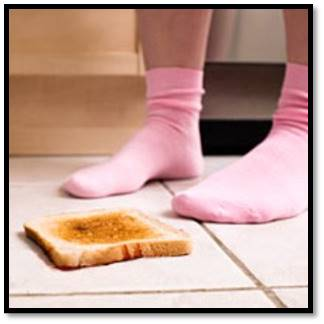
\includegraphics[width=1.00\textwidth]{toast.jpg}
        \label{fig:toast}
      \end{figure}
      
    \end{column}
    \begin{column}{0.3\textwidth}
      
      \begin{figure}
        \centering
        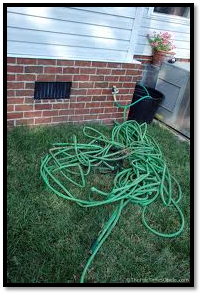
\includegraphics[width=1.00\textwidth]{hose.png}
        \label{fig:hose}
      \end{figure}
      
    \end{column}
    \begin{column}{0.3\textwidth}
      
      \begin{figure}
        \centering
        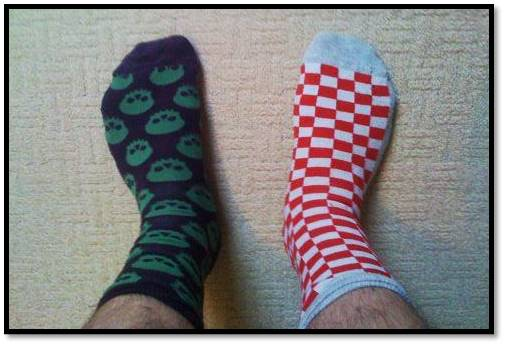
\includegraphics[width=1.00\textwidth]{socks.jpg}
        \label{fig:socks}
      \end{figure}
      
    \end{column}
  \end{columns}
  \note{Students had to investigate whether there is a relationship between a sandwich falling on the butter side and the height a.o, 
  or wether there was a relationship between the number of unpaired socks and other phenomena such as doing your own laundry, exercising often or not \dots}
\end{frame}

\section{Crosstables and Cramér's V}

\begin{frame}
  \frametitle{Crosstables}
  Is there a difference in appreciation by men and women for a particular range of products?
  
  \begin{table}[h]
    \begin{tabular}{l||l|l||l}
                 & Women & Men &  Total \\ \hline \hline
            Good &     9 &   8 &     17 \\
      Sufficient &     8 &  10 &     18 \\
    Insufficient &     5 &   5 &     10 \\
             Bad &     0 &   4 &      4 \\ \hline \hline
           Total &    22 &  27 &     49 \\      
    \end{tabular}
  \end{table}
\end{frame}

\begin{frame}
  \frametitle{Chi-square ($\chi^2$) }
  
  \alertbox{Chi-square ($\chi^2$) is a metric that indicates how much the values in a cross table deviate from the expected values if you assume there is \textit{no} relationship between the two variables.}
  
  \[ \chi^2 = \sum \frac{(o - e)^2}{e} \]
  
  \begin{itemize}
    \item The sum is calculated over all values in the crosstable
    \item $o$: observed value
    \item $e$: expected value
  \end{itemize}
\end{frame}

\begin{frame}
  \frametitle{Crosstables}
  \framesubtitle{Percentages}
  
  \begin{adjustwidth}{-1.5em}{-1.5em}
    \begin{table}[h] \centering
      \begin{tabular}{@{}rrrrrrr@{}} \toprule
                     & Women   & Men  &  Total   & Women \% & Men\%   & Total  \\ \midrule
        Good         & $9$     & $8$  & $17$     & $41$\%  & $30$\%  & $35$\% \\
        Sufficient   & $8$     & $10$ & $18$     & $36$\%  & $37$\%  & $37$\% \\
        Insufficient & $5$     & $5$  & $10$     & $23$\%  & $18$\%  & $20$\% \\
        Bad          & $0$     & $4$  & $4$      & $0$\%   & $15$\%  & $8$\%  \\
        Total        & $22$    & $27$ & $49$     & $100$\% & $100$\% & $100$\%\\
        \bottomrule
      \end{tabular}
    \end{table}
  \end{adjustwidth}
\end{frame}

\begin{frame}
  \frametitle{Crosstable}
  \framesubtitle{Calculate difference $(o - e)$}
  
  \begin{adjustwidth}{-1.5em}{-1.5em}
    \begin{table}[h] \centering
      \begin{tabular}{@{}rrrrrrr@{}} \toprule
        & Women    & Men  &  Total   & Women \% & Men\%   & Total  \\ \midrule
        Good         & $9 -\textcolor{red}{7.63}$     & $8 - \textcolor{red}{9.36}$   & $17$     & $41$\%  & $30$\% & $35$\% \\
        Sufficient   & $8 - \textcolor{red}{8.08}$   & $10 - \textcolor{red}{9.91}$  & $18$     & $36$\%  & $37$\%    & $37$\% \\
        Insufficient & $5 - \textcolor{red}{4.48}$    & $5 - \textcolor{red}{5.51}$  & $10$     & $23$\%  & $18$\% & $20$\% \\
        Bad          & $0 - \textcolor{red}{1.79}$    & $4 - \textcolor{red}{2.20}$  & $4$      & $0$\%      & $15$\% & $8$\%  \\
        Total        & $22$    & $27$  & $49$     & $100$\%    & $100$\%   & $100$\%   \\
        \bottomrule
      \end{tabular}
    \end{table}
  \end{adjustwidth}
\end{frame}

\begin{frame}
  \frametitle{Crosstables}
  \framesubtitle{Square and normalize $\frac{(o-e)^2}{e}$}
  
  \begin{table}[h] \centering
    \begin{tabular}{@{}rrrrrrr@{}} \toprule
      & Women    & Men  &  Total   & Women \% & Men\%   & Total  \\
      \midrule
      Good         & $\textcolor{blue}{0.2}$ & $\textcolor{blue}{0.2}$ & $17$   & $41$\%   & $30$\%  & $35$\% \\
      Sufficient   & $\textcolor{blue}{0}$   & $\textcolor{blue}{0}$   & $18$   & $36$\%   & $37$\%  & $37$\% \\
      Insufficient & $\textcolor{blue}{0.1}$ & $\textcolor{blue}{0}$   & $10$   & $23$\%   & $18$\%  & $20$\% \\
      Bad          & $\textcolor{blue}{1.8}$ & $\textcolor{blue}{1.5}$ & $4$    & $0$\%    & $15$\%  & $8$\%  \\
      Total        & $22$                    & $27$                    & $49$   & $100$\%  & $100$\% & $100$\%   \\
      \bottomrule
    \end{tabular}
  \end{table}
  \[ \chi^{2} = 3.811, V= 0.279 \]
\end{frame}

\section{Cramér's V}

\begin{frame}
  \frametitle{Cramér's V}
  
  \alertbox{Cramér's V is a measure that indicates how strong the relationship is between two qualitative variables. Its value is always between 0 and 1}
  
  \[ V = \sqrt{\frac{\chi^2}{n (k - 1)}} \]
  
  $n$: number of observations
  
  $k$: min(number of rows, number of columns)
\end{frame}

\begin{frame}
  \frametitle{Interpretation Cramér's V}
  
  \begin{table}[h] \centering
    \begin{tabular}{@{}rr@{}} \toprule
      Value & Interpretation \\
      \midrule
      $0$ & no association \\
      $0.1$ &  weak association \\
      $0.25$ & fairly strong association \\
      $0.5$ & strong association \\
      $0.75$ & very strong association \\
      $1$ & complete association \\
      \bottomrule
    \end{tabular}
  \end{table}
\end{frame}

\begin{frame}
  \frametitle{Example 2}
  \framesubtitle{Relationship between gender and preference for a particular car brand}
  
  \begin{table}[h] \centering
    \begin{tabular}{@{}rrrrrr@{}} \toprule
      & Mercedes & BMW & Porsche& Alfa Romeo & Total \\
      \midrule
      Men     & $10$ & $10$ & $20$ & $20$ & $60$ \\
      Women   & $20$ & $5$  & $15$ & $0$  & $40$ \\
      Total   & $30$ & $15$ & $35$ & $20$ & $100$ \\
      \bottomrule
    \end{tabular}
  \end{table}
  It seems as if the different car brands are not equally valued by men and women.
  \[ \chi^{2} = 22.619, V = \sqrt{\frac{22.169}{100 . (2-1)}}  = 0.476\]
\end{frame}


\section{Chi-square test for a single variable}

\begin{frame}
  \frametitle{Goodness of fit test}
  \alertbox{A \textcolor{hgyellow}{goodness of fit test} indicates to what degree a sample corresponds to a null hypothesis regarding the distribution of a qualitative variable.}
  
  \begin{columns}
    \begin{column} {0.35\textwidth}
      
      \begin{figure}
        \centering
        
\includegraphics[height=.5\textheight]{les6-man.jpg}
      \end{figure}
      
    \end{column}
    \begin{column} {0.65\textwidth}
      
      \begin{figure}
        \centering
        
\includegraphics[height=.5\textheight]{les5-heroes.jpg}
      \end{figure}
      
    \end{column}
  \end{columns}
\end{frame}

\begin{frame}
  \frametitle{Goodness of fit test}
  \begin{columns}
    \begin{column} {0.2 \textwidth}
      
      \begin{figure}
        \centering
        
\includegraphics[width=\textwidth]{les6-man.jpg}
      \end{figure}
      
    \end{column}
    
    \begin{column} { 0.8 \textwidth}
      \begin{table}[h]
        \begin{tabular}{@{}lcc@{}}
          \toprule
          \textbf{Type}   & \textbf{\# sample}     & \textbf{\# population} \\ \midrule
          Mutant          &          127           &         35\%           \\
          Human           &           75           &         17\%           \\
          Alien           &           98           &         23\%           \\
          God             &           27           &          8\%           \\
          Demon           &           73           &         17\%           \\ \midrule
          \textbf{Total}  &          400           &         100\%          \\
        \end{tabular}
      \end{table}
    \end{column}
  \end{columns}
\end{frame}

\begin{frame}
  \frametitle{Goodness of fit test}
  Is the distribution of the sample ($n = 400$) representative for the full population (all superheroes)?
  
  \begin{itemize}
    \item What numbers would you \textit{expect} if the sample is representative?
    \item How large are the differences from the \textit{observed} numbers?
    \begin{itemize}
      \item small $\Rightarrow$ distribution is representative
      \item large $\Rightarrow$ distribution is \textbf{not} representative
    \end{itemize}
  \end{itemize}
  
  \pause
  Can you see the link between crosstables and Cramer's V?
\end{frame}

\begin{frame}
  \frametitle{Notation}
  
  In the next slides is:
  
  \begin{itemize}
    \item $e$ the \textit{expected} frequency for a category
    \item $\pi$ the expected \textit{relative frequency} for a category (percentage)
    \item $o$ the \textit{observed} absolute frequency
    \item $n$ the sample size (as usual)
    \item $i$ an index indicating a category in the frequency table ($i \in \{1, \ldots, k\}$)
  \end{itemize}
\end{frame}

\begin{frame}
  \frametitle{Goodness of fit test}
  \begin{itemize}
    \item Exactly representative $\Rightarrow$ 35\% of superheroes in the sample is a mutant
    \item The expected number therefore is $e = 0.35 \times 400 = 140$.
  \end{itemize}
  Therefore:
  
  \[ e = n \times \pi \]
  
  If the differences $o - e$ are relatively small they can be attributed to random sampling errors. 
\end{frame}

\begin{frame}
  \frametitle{Goodness of fit test}
  Consider $\chi^{2}$:
  
  \[ \chi^{2} = \sum_{i=1}^{n} \frac{(o_{i} - e_{i})^{2}}{e_{i}} \]
  
  Draw a conclusion based on the value of $\chi^2$:
  \begin{itemize}
    \item small $\Rightarrow$ distribution is representative
    \item large $\Rightarrow$ distribution is \textbf{not} representative
  \end{itemize}
  
  $\chi^{2}$ measures the degree of conflict with the null hypothesis
\end{frame}

\begin{frame}
  \frametitle{Goodness of fit test}
  \begin{columns}
    \begin{column} {0.2 \textwidth}
      
      \begin{figure}
        \centering
        
\includegraphics[width=\textwidth]{les6-man.jpg}
      \end{figure}
      
    \end{column}
    
    \begin{column} { 0.8 \textwidth}
      % Please add the following required packages to your document preamble:
      % \usepackage{booktabs}
      \begin{table}[h]
        \begin{tabular}{@{}llllll@{}}
          \toprule
          \textbf{Superhero type} & \textbf{$o$} & \textbf{$\pi$} & \textbf{$e$} & \textbf{$o -e$} & \textbf{$\frac{(o-e)^{2}}{e}$} \\ \midrule
          Mutant                  & 127          & 35\%           & 140          & -13             & 1.21                           \\
          Human                   & 75           & 17\%           & 68           & 7               & 0.72                           \\
          Alien                   & 98           & 23\%           & 92           & 6               & 0.39                           \\
          God                     & 27           & 8\%            & 32           & -5              & 0.78                           \\
          Demon                   & 73           & 17\%           & 68           & 5               & 0.37                           \\ \bottomrule
        \end{tabular}
      \end{table}
    \end{column}
  \end{columns}
\end{frame}


\begin{frame}
  \frametitle{Goodness of fit test}
  
  \begin{itemize}
    \item The test statistic $\chi^{2}$ follows the $\chi^2$ distribution.
    \item Critical value $g$ from the $\chi^{2}$ distribution: this is dependent on the number of degrees of freedom ($df$). In general:
    
    \[ df = k -1 \]
    
    \item The critical value $g$ for a given significance level $\alpha$ and number of degrees of freedom $df$ can be calculated in R using the function `qchisq()`.
    
    \[ P(\chi^2 < g) = 1 - \alpha \]
  \end{itemize}
\end{frame}

\begin{frame}[fragile]
  \frametitle{Goodness of fit test}
  \framesubtitle{Calculate critical value}
  
  \begin{itemize}
    \item Suppose $\alpha = 0.05$ and $df = 5 - 1 = 4$
    \item \verb|g <- qchisq(0.95, df = 4)|, so $g = 9.49$
    \item $\chi^{2} = 3.47 < g = 9.49$
    \item Conclusion: the sample is representative ($H_0$ is accepted)
  \end{itemize}
\end{frame}

\begin{frame}[fragile]
  \frametitle{Goodness of fit test}
  \framesubtitle{Calculate probability value}
  
  You can also calculate the probability value:
  
  \[ p = P(X > \chi^2) = 1 - P(X < \chi^2) \]
  
  \begin{itemize}
    \item \verb|p <- 1 - pchisq(3.47, df = 4)|, so $p = 0.48$
    \item $p = 0.48 < \alpha = 0.05$
    \item Conclusion: the sample is representative ($H_0$ is accepted)
  \end{itemize}
\end{frame}

\subsection{Testing procedure for goodness of fit test}

\begin{frame}
  \frametitle{Goodness of fit test}
  \framesubtitle{Testing Procedure}
  
  \begin{enumerate}
    \item \textbf{Formulate both hypotheses}
    \begin{itemize}
      \item $H_{0}$: sample is representative for the population
      \item $H_{1}$: sample is not representative for the population
    \end{itemize}
    \item \textbf{Determine $\alpha$ and $n$} : $\alpha = 0.05$ and $n = 400$.
  \end{enumerate}
\end{frame}

\begin{frame}
  \frametitle{Goodness of fit test}
  \framesubtitle{Testing Procedure}
  
  \begin{enumerate}
    \item \textbf{Calculate test statistic}:
    \[ \chi^{2} = \sum_{i=1}^{n} \frac{(o_{i} - e_{i})^{2}}{e_{i}} \]
    \item 
    \begin{enumerate}
      \item \textbf{Critical area}: Calculate $g$ so that $P(\chi^2 < g) = 1 - \alpha$
      \item \textbf{Probability value}: Calculate $p = 1 - P(X < \chi^2)$
    \end{enumerate}
    
    \item Conclusion (the test is always right-tailed):
    \begin{enumerate}
      \item $\chi^2 < g \Rightarrow$ do not reject $H_0$
      \item $p > \alpha \Rightarrow$ reject $H_0$, accept $H_1$
    \end{enumerate}
  \end{enumerate}
\end{frame}


\subsection{Example}

\begin{frame}
  \frametitle{Example: families}
  Consider all families with exactly 5 children in a given community.
  \pause
  When we look at the number of boys/girls, there are 6 possible combinations:
  \begin{enumerate}
    \item 5 boys
    \item 4 boys, 1 girl
    \item 3 boys, 2 girls
    \item 2 boys, 3 girls
    \item 1 boy, 4 girls
    \item 5 girls
  \end{enumerate}
  A survey was conducted regarding 1022 families with exactly 5 children
  \begin{center}
    Are the observed numbers in the 6 classes representative for a population in which the probability of having a boy is equal to the probability of having a girl, or more concrete 0.5?
  \end{center}
\end{frame}

\begin{frame}
  \frametitle{Example}
  \begin{table}[h]
    \begin{tabular}{@{}llllllll@{}}
      \toprule
      i       & 0  & 1   & 2   & 3   & 4   & 5  &  \\ \midrule
      $o_{i}$ & 58 & 149 & 305 & 303 & 162 & 45 &  \\ \bottomrule
    \end{tabular}
  \end{table}
  \pause
  If the assumption is true, the probability $\pi_{i}$ to have $i$ boys is determined by a binomial distribution with parameters $n=5$ and $p=0.5$.
  For example, the probability to have 2 boys out of 5 children is equal to:
  
  \[ (0.5)^{2} \times (1-0.5)^{5-2} \times \binom{5}{2} \]
  
  In general:
  
  \[ \pi_{i} = \binom{5}{i}\times 0.5^{i} \times 0.5^{5-i} = \frac{5!}{i!(5-i)!}\times 0.5^{i} \]
\end{frame}

\begin{frame}
  \frametitle{Example}
  \centering
  \begin{tabular}{lSSSSSSS}
    \toprule
    $i$                   & 0      & 1      & 2      & 3      & 4     & 5     & Totaal \\
    \midrule
    $o_i$                 & 58     & 149    & 305    & 303    & 162   & 45    & 1022   \\
    $\pi_i$               & 0,031  & 0,156  & 0,313  & 0,313  & 0,156 & 0,031 & 1      \\
    $e_i$                 & 31,9   & 159,7  & 319,4  & 319,4  & 159,7 & 31,9  & 1022   \\
    $\frac{(o-e)^{2}}{e}$ & 21,268 & 0,715  & 0,647  & 0,840  & 0,033 & 5,343 & 28,846 \\
    $r_i$                 & 4,686  & -0,921 & -0,970 & -1,105 & 0,199 & 2,348 &        \\
    \bottomrule
  \end{tabular}
\end{frame}

\begin{frame}
  \frametitle{Example}
  \begin{enumerate}
    \item \textbf{Formulate both hypotheses}
    \begin{itemize}
      \item $H_{0}$: the sample is representative for the population
      \item $H_{1}$: the sample is not representative for the population
    \end{itemize}
    \item \textbf{Determine $\alpha$ and $n$} : $\alpha = 0.01$ and $n = 1022$.
    \item \textbf{Value of the test statistic in the sample}:
    \[ \chi^{2} = \sum_{i=1}^{n} \frac{(o_{i} - e_{i})^{2}}{e_{i}} \approx 28.846 \]
    \item \textbf{Calculate and plot critical area}:  The critical value is $15.0863$. Our test statistic is inside the critical area, so we can reject $H_{0}$.
  \end{enumerate}
\end{frame}

\subsection{Standardized Residuals}
\begin{frame}
  \frametitle{Standardized Residuals}
  \alertbox{The \textcolor{hgyellow}{standardized residuals} indicate which classes make the greatest contribution to the value of $\chi^2$.}
  \[ r_{i} = \frac{o_{i} - n \pi_{i}}{\sqrt{n \pi_{i}(1-\pi_{i})}} \]
  
  \begin{itemize}
    \item In general, values greater than 2 or less than $-2$ are extreme.
  \end{itemize}
  We can therefore conclude that the number of families in which all children are of the same gender can be called larger than expected.
  
\end{frame}

\begin{frame}
  \frametitle{Conditions}
  In order to apply the $\chi^2$-test, the following conditions must be met (Rule of Cochran)
  \begin{enumerate}
    \item For all categories, the expected frequency $e$ must be greater than 1.
    \item In a maximum of 20 \% of the categories, the expected frequency $e$ may be less than 5.
  \end{enumerate}
\end{frame}

\section{Chi-square test for two variables}

\begin{frame}
  \frametitle{$\chi^{2}$ test for two variables}
  The chi-square test can be easily extended for two variables, which respectively have $r$ and $k$ levels.
\end{frame}

\begin{frame}
  \frametitle{Study about smoking}
  In this study, Doll and Hill investigated the relationship between smoking and lung cancer. In 1951, Doll and Hill wrote to all British general practitioners (GPs) requesting information about their age and smoking behavior. Next, they tracked death reports and cause of death over years and repeated this periodically. The first results, after around four years, are summarized in the table below.  
  
  \begin{table}[h]
    \begin{tabular}{@{}lllll@{}}
      \toprule
      & \textbf{Lung Cancer} & \textbf{No} & \textbf{Yes} & \textbf{Total} \\ \midrule
      \textbf{Smoker} & \textbf{Yes}        & 21178         & 83           & 21261           \\
                      & \textbf{No}         & 3092          & 1            & 3093            \\
                      & \textbf{Total}      & 24270         & 84           & 24354           \\ \bottomrule
    \end{tabular}
  \end{table}
\end{frame}

\begin{frame}
  \frametitle{Study about smoking}
  \begin{table}[h]
    \begin{tabular}{@{}lllll@{}}
      \toprule
      & \textbf{Lung Cancer} & \textbf{No} & \textbf{Yes} & \textbf{Total} \\ \midrule
      \textbf{Smoker} & \textbf{Yes}        & 21178         & 83           & 21261           \\
      & \textbf{No}         & 3092          & 1            & 3093            \\
      & \textbf{Total}      & 24270         & 84           & 24354           \\ \bottomrule
    \end{tabular}
  \end{table}
  
  \begin{columns}
    \begin{column}{0.3 \textwidth}
      
      \begin{figure}
        \centering
        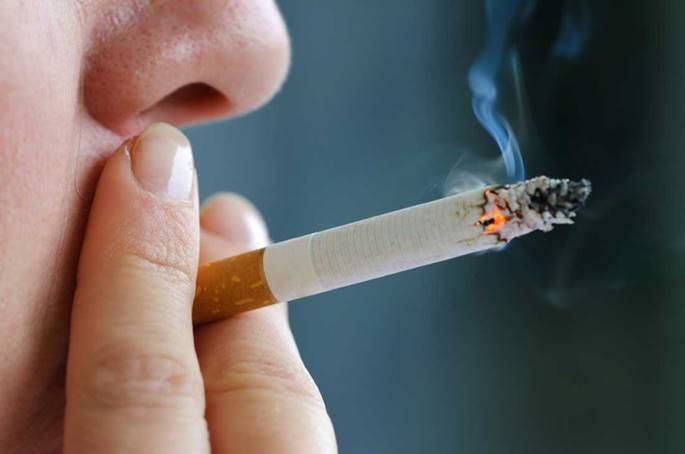
\includegraphics[width=1.00\textwidth]{les-6-smoking.jpg}
      \end{figure}
      
    \end{column}
    \begin{column}{0.7 \textwidth}
      
      \begin{itemize}
        \item \dots only $\frac{84}{ 24354} \times 100 = 0.35\% $ of British GPs died of lung cancer
        \item \dots with only $\frac{83}{21261} \times 100 = 0.39\%$ of smokers among them
        \item \dots but this results is much larger than the result for the non-smokers $\frac{1}{3093} * 100 = 0.032\%$.
      \end{itemize}
    \end{column}
  \end{columns}
\end{frame}

\begin{frame}
  \frametitle{Study about smoking}
  % Please add the following required packages to your document preamble:
  % \usepackage{booktabs}
  \begin{table}[h]
    \begin{tabular}{@{}lllll@{}}
      \toprule
      & \textbf{Lung Cancer} & \textbf{No} & \textbf{Yes} & \textbf{Total} \\ \midrule
      Smoker & Yes                 & 21188         & 73.3         & 21261           \\
      & No                & 3082.3        & 10.7         & 3093            \\
      & Total              & 24270         & 84           & 24354           \\ \bottomrule
    \end{tabular}
  \end{table}
  
  \begin{columns}
    \begin{column}{0.3 \textwidth}
      
      \begin{figure}
        \centering
        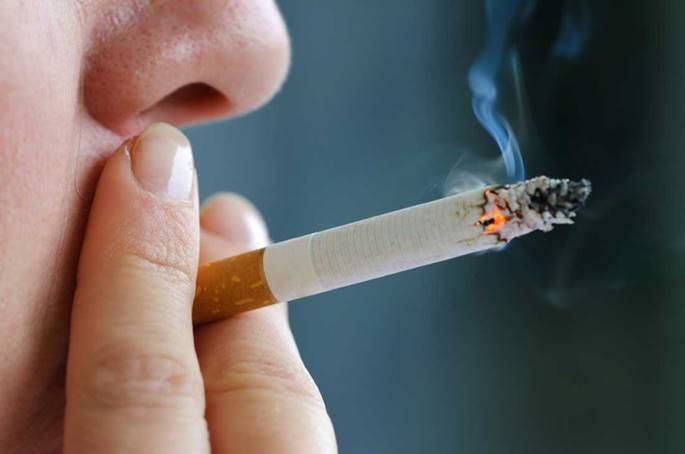
\includegraphics[width=1.00\textwidth]{les-6-smoking.jpg}
      \end{figure}
      
    \end{column}
    \begin{column}{0.7 \textwidth}
      
      \begin{itemize}
        \item $\chi^{2} = 10.35$
        \item We can see from the table that there is a large difference between the observed number of smoker that died of lung cancer and the expected values of the cell.
        \item The same is true for the limited number of GPs that doesn't smoke, but died of lung cancer.
      \end{itemize}
    \end{column}
  \end{columns}
\end{frame}

\begin{frame}
  \frametitle{Study about smoking}
  \begin{enumerate}
    \item \textbf{Formulate both hypotheses}
    \begin{itemize}
      \item $H_{0}$: in the population there is no relationship between the independent and dependent variable
      \item $H_{1}$: there is a relationship 
    \end{itemize}
    \item \textbf{Determine $\alpha$ and $n$} : $\alpha = 0.05$ en $n = 24354$.
    \item \textbf{Calculate the value of the test statistic in the sample}:
    \[ \chi^{2} = \sum_{i=1}^{n} \frac{(o_{i} - e_{i})^{2}}{E_{i}} = 10.35 \]
    \item \textbf{Calculate and plot the critical region}:  the critical value is 3.8415 and the number of degrees of freeodm $df = (r-1)(k-1)$. Our test statistic is inside the critical region so we reject $H_{0}$.
  \end{enumerate}
\end{frame}

\begin{frame}
  \frametitle{Causal relationship}
  We therefore have to reject $H_{0}$, which states that there is no relationship between both variables, in favor of $H_{1}$ which states that there is a relationship: smokers are more likely to die of lung cancer compared to non-smokers.
  \begin{columns}
    \begin{column}{0.3 \textwidth}
      
      \begin{figure}
        \centering
        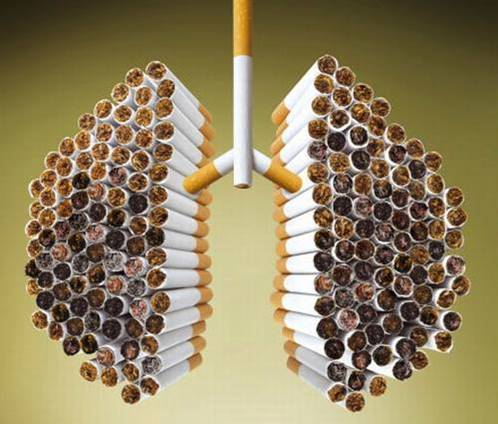
\includegraphics[width=1.00\textwidth]{les-6-smoking2.jpg}
      \end{figure}
      
    \end{column}
    \begin{column}{0.7 \textwidth}
      
      \begin{itemize}
        \item  \dots smokers are older than non-smokers
        \item \dots smokers often live in large cities with more polluted air than non-smokers
        \item \dots a special genetic disposition affects both tobacco addiction as well as the chance of developing lung cancer
      \end{itemize}
    \end{column}
  \end{columns}
  For a causal interpretation of the data (note, after all, this is not an experiment), we should at least have a theory that makes the relationship between smoking and lung cancer explicit.
  
\end{frame}

\section{Graphs for crosstables}

\begin{frame}
  \frametitle{Visualization of crosstables}
  
  \begin{figure}
    \centering
    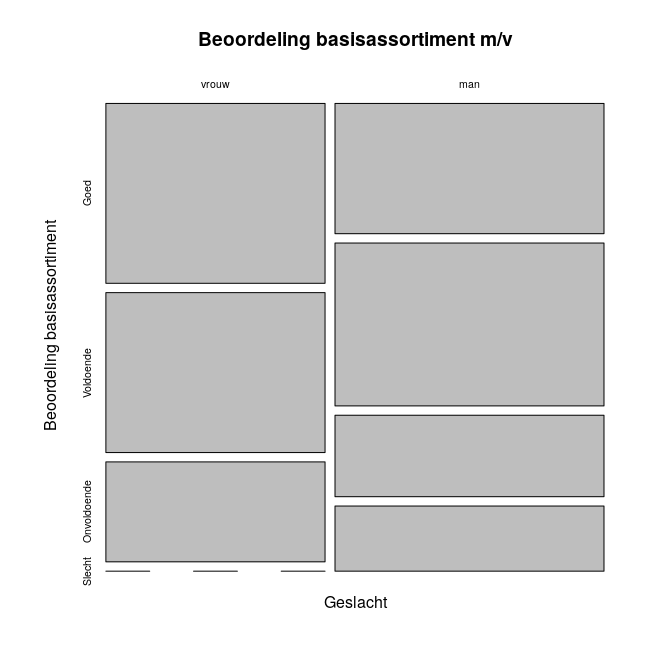
\includegraphics[height=.8\textheight]{2var-xtab-plot-waardering}
  \end{figure}
  
\end{frame}

\begin{frame}
  \frametitle{Visualization of crosstables}
  \framesubtitle{Clustered bar chart}
  
  \begin{figure}
    \centering
    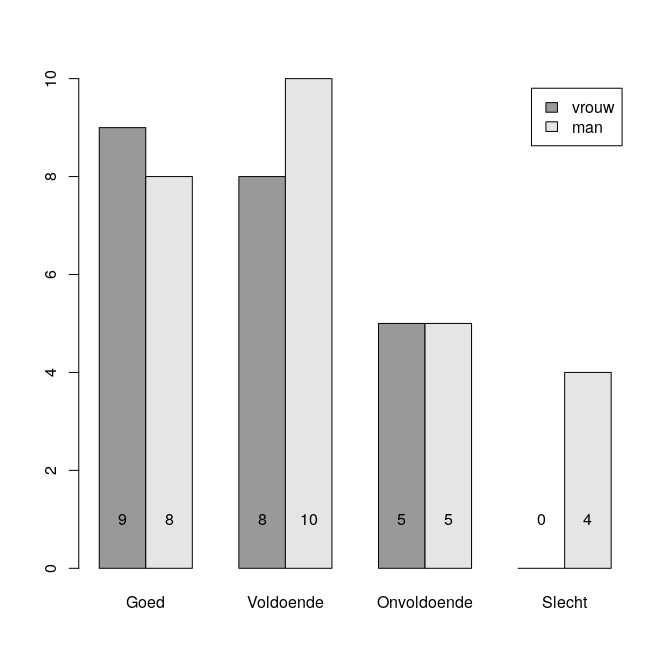
\includegraphics[height=.8\textheight]{2var-staafgrafiek-geclusterd}
  \end{figure}
  
\end{frame}

\begin{frame}
  \frametitle{Visualization of crosstables}
  \framesubtitle{Horizontal stacked bar chart}
  
  \begin{figure}
    \centering
    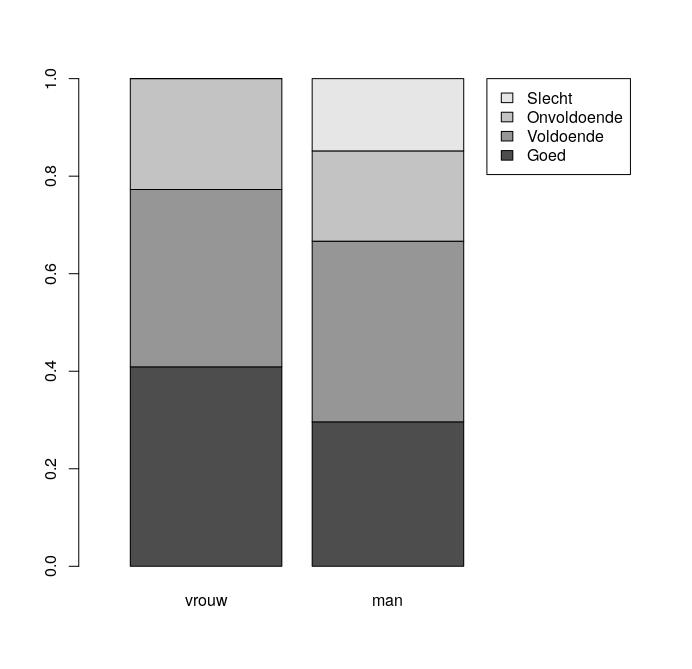
\includegraphics[height=.8\textheight]{2var-rependiagram-waardering-mv}
  \end{figure}
  
\end{frame}

\end{document}